\documentclass{beamer}

\usepackage{cmap}				% To be able to copy-paste russian text from pdf
\usepackage[T2A]{fontenc}
\usepackage[utf8]{inputenc}
\usepackage[english]{babel}
\usepackage{textpos}
\usepackage{ragged2e}
\usepackage{amssymb}
\usepackage{ulem}
\usepackage{tikz}
\usepackage{pgfplots}
\usepackage{color}
\usepackage{cancel}
\usepackage{multirow}
\pgfplotsset{compat=1.17}
\usetikzlibrary{arrows,snakes,backgrounds,shapes}
\usepgfplotslibrary{groupplots,colorbrewer,dateplot,statistics}
\usepackage{animate}

\usepackage{amsfonts}
\usepackage{amsmath}
\usepackage{amssymb}
\usepackage{graphicx}
\usepackage{setspace}
\usepackage{tabularx}

\usepackage{enumitem}
\setitemize{label=\usebeamerfont*{itemize item}%
  \usebeamercolor[fg]{itemize item}
  \usebeamertemplate{itemize item}}

% remove navigation bar
\setbeamertemplate{navigation symbols}{} 

\setbeamertemplate{page number in head/foot}[totalframenumber] 

\usepackage{eurosym}
\renewcommand{\EUR}[1]{\textup{\euro}#1}

\title{Monte Carlo Method}
\author{Artem Bakulin}
\date{November 23, 2023}

\usetheme{Warsaw}
\usecolortheme{beaver}

% https://tex.stackexchange.com/questions/98003/filter-rows-from-a-table
\pgfplotsset{
    discard if not/.style 2 args={
        x filter/.code={
            \edef\tempa{\thisrow{#1}}
            \edef\tempb{#2}
            \ifx\tempa\tempb
            \else
                \def\pgfmathresult{inf}
            \fi
        }
    }
}



\begin{document}



\begin{frame}
\titlepage
\end{frame}



\newcommand{\drawStockNode}[5]{

	\node (#5)
	[
		draw,
		rectangle,
		rounded corners,
		inner sep = 0pt,
		outer sep = 0pt,
		minimum width = 2.4cm,
		minimum height = 0.55cm,
		align = center
	]
	at (#3, #4)
	{
		\begin{tabular}{c|c}
		#1 & #2
		\end{tabular}
	};
}

\newcommand{\drawStockLink}[4]{

	\draw[
		->,
		>=triangle 90
	]
	(#1.east) -- (#2.west)
	node[
		pos = 0.5,
		anchor = #4
	]
	{#3};
}

\newcommand{\drawOneStepBinomialTree}{
	\drawStockNode{$S_0$} {?}{0}{ 0}{S0_node}
	\drawStockNode{$S_0u$}{$V_u$}{4}{ 1}{Su_node}
	\drawStockNode{$S_0d$}{$V_d$}{4}{-1}{Sd_node}
	
	\drawStockLink{S0_node}{Su_node}{$p$}{south east}	
	\drawStockLink{S0_node}{Sd_node}{$1-p$}{north east}
}



\begin{frame}{Recap: binomial model}
\centering
\begin{tikzpicture}
	\drawOneStepBinomialTree
\end{tikzpicture}

\justify
\begin{itemize}
\justifying
\item Current stock price is $S_0$.
\item Stock price can either increase to $S_0\cdot u$ (u>1) or drop to $S_0 \cdot d$ (d<1).
\item Single period of $\tau$ years, risk-free interest rate is $r$, such that $d < 1+r\tau < u$.
\item An option pays off (has the value of) either $V_u$ or $V_d$ depending on the stock price moving up or down.
\end{itemize}
\end{frame}



\begin{frame}{Recap: binomial model - 2}
\centering
\begin{tikzpicture}
	\drawOneStepBinomialTree
\end{tikzpicture}

\justify
Consider a portfolio of $\Delta$ stock and debt $L$. Pick $\Delta$ and $L$ so that this portfolio replicates the option
\begin{equation*}
\begin{cases}
L(1+r\tau) + \Delta S_0 u = V_u \\
L(1+r\tau) + \Delta S_0 d = V_d
\end{cases}
\end{equation*}

\begin{equation*}
\begin{cases}
\Delta = \dfrac{V_u - V_d}{S_0(u-d)} \\
L = \dfrac{V_du - V_ud}{(1+r\tau)(u-d)}
\end{cases}
\end{equation*}
\end{frame}



\begin{frame}{Recap: binomial model - 3}
\centering
\begin{tikzpicture}
\drawOneStepBinomialTree
\end{tikzpicture}

\justify
The option is worth the same as the replicating portfolio:
\begin{align*}
C &= \Delta S_0 +L = \\
 &= \dfrac{V_u-V_d}{(u-d)\cancel{S_0}}\cancel{S_0} + \dfrac{V_du -V_ud}{(1+r\tau)(u-d)} = \\
 &= \dfrac{qV_u +(1-q)V_d}{1+r\tau},
\end{align*}
where
\begin{equation*}
q = \dfrac{1+r\tau - d}{u-d}
\end{equation*}
This magic parameter $q$ is called the "risk-neutral probability".
\end{frame}



\renewcommand{\drawStockLink}[2]{

	\draw[
		->,
		>=triangle 45
	]
	(#1.east) -- (#2.west)
	{};
}

\renewcommand{\drawStockNode}[5]{

	\node (#5)
	[
		draw,
		rectangle,
		rounded corners,
		inner sep = 1pt,
		outer sep = 0pt,
		minimum width = 1.5cm
	]
	at (#3, #4)
	{
		\centering
		\begin{tabular}{c}
		#1 \\ \hline #2
		\end{tabular}
	};
}

\newcommand{\nodeVerticalStep}{0.7}
\newcommand{\nodeHorizontalStep}{2.75}

\begin{frame}{Recap: binomial model - 4}
\centering
\begin{tikzpicture}
\drawStockNode{$\$100$}{\only<1-7>{?}\only<8->{\$14.8}}{0}{0}{S0_node}

\drawStockNode{$\$120$}{\only<1-5>{?}\only<6->{\$25.8}}{\nodeHorizontalStep}{\nodeVerticalStep}{Su_node}
\drawStockNode{$\$80$}{\only<1-6>{?}\only<7->{\$3.8}}{\nodeHorizontalStep}{-\nodeVerticalStep}{Sd_node}

\drawStockNode{$\$144$}{\only<1-2>{?}\only<3->{\$44}}{2*\nodeHorizontalStep}{2*\nodeVerticalStep}{Suu_node}
\drawStockNode{$\$96$}{\only<1-3>{?}\only<4->{\$7.6}}{2*\nodeHorizontalStep}{0}{Sud_node}
\drawStockNode{$\$64$}{\only<1-4>{?}\only<5->{\$0}}{2*\nodeHorizontalStep}{-2*\nodeVerticalStep}{Sdd_node}

\drawStockNode{$\$172.8$}{\only<1>{?}\only<2->{\$72.8}}{3*\nodeHorizontalStep}{3*\nodeVerticalStep}{Suuu_node}
\drawStockNode{$\$115.2$}{\only<1>{?}\only<2->{\$15.2}}{3*\nodeHorizontalStep}{\nodeVerticalStep}{Suud_node}
\drawStockNode{$\$76.8$}{\only<1>{?}\only<2->{\$0}}{3*\nodeHorizontalStep}{-\nodeVerticalStep}{Sudd_node}
\drawStockNode{$\$51.2$}{\only<1>{?}\only<2->{\$0}}{3*\nodeHorizontalStep}{-3*\nodeVerticalStep}{Sddd_node}

\drawStockLink{S0_node}{Su_node}
\drawStockLink{S0_node}{Sd_node}

\drawStockLink{Su_node}{Suu_node}
\drawStockLink{Su_node}{Sud_node}

\drawStockLink{Sd_node}{Sud_node}
\drawStockLink{Sd_node}{Sdd_node}

\drawStockLink{Suu_node}{Suuu_node}
\drawStockLink{Suu_node}{Suud_node}

\drawStockLink{Sud_node}{Suud_node}
\drawStockLink{Sud_node}{Sudd_node}

\drawStockLink{Sdd_node}{Sudd_node}
\drawStockLink{Sdd_node}{Sddd_node}
\end{tikzpicture}

\justify
Suppose that $u=1.2$, $d=0.8$, $S_0=\$100$, $r=0\%$. What is fair value of a call option at strike $K=100$?

\justify
The "risk-neutral probability":
\begin{align*}
q = \dfrac{1+r\tau - d}{u - d} = \dfrac{1 - 0.8}{1.2 - 0.8} = 0.5
\end{align*}
\end{frame}





\newcommand{\highlightStockLink}[6]{
	\draw[
		color=#4,
		very thick,
		->,
		>=triangle 45
	]
	(#1.east) -- (#2.west)
	node[
		pos=#5,
		anchor=#6
	]
	{#3};
}

\newcommand{\highlightStockLinkUp}[3]{
	\highlightStockLink{#1}{#2}{$q$}{#3}{0.5}{south}
}

\newcommand{\highlightStockLinkDown}[3]{
	\highlightStockLink{#1}{#2}{$1-q$}{#3}{0.15}{west}
}

\begin{frame}{Recap: risk-neutral probability}
\centering
\begin{tikzpicture}
\drawStockNode{$S_0$}{?}{0}{0}{S0_node}

\drawStockNode{$S_0u$}{?}{\nodeHorizontalStep}{\nodeVerticalStep}{Su_node}
\drawStockNode{$S_0d$}{?}{\nodeHorizontalStep}{-\nodeVerticalStep}{Sd_node}

\drawStockNode{$S_0u^2$}{?}{2*\nodeHorizontalStep}{2*\nodeVerticalStep}{Suu_node}
\drawStockNode{$S_0ud$}{?}{2*\nodeHorizontalStep}{0}{Sud_node}
\drawStockNode{$S_0d^2$}{?}{2*\nodeHorizontalStep}{-2*\nodeVerticalStep}{Sdd_node}

\drawStockNode{$S_0u^3$}{$V_3$}{3*\nodeHorizontalStep}{3*\nodeVerticalStep}{Suuu_node}
\drawStockNode{$S_0u^2d$}{$V_2$}{3*\nodeHorizontalStep}{\nodeVerticalStep}{Suud_node}
\drawStockNode{$S_0ud^2$}{$V_1$}{3*\nodeHorizontalStep}{-\nodeVerticalStep}{Sudd_node}
\drawStockNode{$S_0d^3$}{$V_0$}{3*\nodeHorizontalStep}{-3*\nodeVerticalStep}{Sddd_node}

\only<1-2>{
	\drawStockLink{S0_node}{Su_node}
	\drawStockLink{S0_node}{Sd_node}

	\drawStockLink{Su_node}{Suu_node}
	\drawStockLink{Su_node}{Sud_node}

	\drawStockLink{Sd_node}{Sud_node}
	\drawStockLink{Sd_node}{Sdd_node}

	\drawStockLink{Suu_node}{Suuu_node}
	\drawStockLink{Suu_node}{Suud_node}

	\drawStockLink{Sud_node}{Suud_node}
	\drawStockLink{Sud_node}{Sudd_node}

	\drawStockLink{Sdd_node}{Sudd_node}
	\drawStockLink{Sdd_node}{Sddd_node}
}

\only<3>{
	\highlightStockLinkUp{S0_node}{Su_node}{Set1-A}
	\highlightStockLinkUp{Su_node}{Suu_node}{Set1-A}
	\highlightStockLinkDown{Suu_node}{Suud_node}{Set1-A}
}

\only<4>{
	\highlightStockLinkUp{S0_node}{Su_node}{Set1-A}
	\highlightStockLinkDown{Su_node}{Sud_node}{Set1-A}
	\highlightStockLinkUp{Sud_node}{Suud_node}{Set1-A}
}

\only<5>{
	\highlightStockLinkDown{S0_node}{Sd_node}{Set1-A}
	\highlightStockLinkUp{Sd_node}{Sud_node}{Set1-A}
	\highlightStockLinkUp{Sud_node}{Suud_node}{Set1-A}
}

\end{tikzpicture}

\justify
Risk-neutral probability: $q = \dfrac{1 + rT - d}{u - d}$.

\justify
Fair value of an option today:
\begin{align*}
V = \frac{q^3V_3 + \only<1>{3q^2(1-q)}\only<2->{\alert{3q^2(1-q)}}V_2 + 3q(1-q)^2V_1 + (1-q)^3V_0}{(1+rT)^3}
\end{align*}
\end{frame}


\begin{frame}{Recap: risk-neutral probability - 2}
\justify
Close your eyes and pretend that $q$ is the probability of the sock price moving up (in reality it is not). Then $3q^2(1-q)$ is probability of the stock moving up twice and moving down once. In this scenario the stock is worth  $S_0u^2d$, and the option pays off $V_2$.

\justify
\centering
\begin{tabular}{l|l|l}
Stock price & Payoff & "Probability" \\ \hline
$S_0u^3$   & $V_3$   & $q^3$ \\
$S_0u^2d$  & $V_2$   & $3q^2(1-q)$ \\
$S_0ud^2$  & $V_1$   & $3q(1-q)^2$ \\ 
$S_0d^3$   & $V_0$   & $(1-q)^3$ 
\end{tabular}

\justify
Fair value of an option looks similar to the discounted "expected"\ payoff.
\begin{align*}
V = \frac{q^3V_3 + 3q^2(1-q)V_2 + 3q(1-q)^2V_1 + (1-q)^3V_0}{(1+rT)^3}
\end{align*}
\end{frame}



\begin{frame}{Stock price}
\justify
A stock is equivalent to a call option at strike 0. This option's terminal payoff is  $V(S) = \max(S-0, 0) = S$.
\begin{align*}
S &= \frac{q^3S_0u^3 + 3q^2(1-q)S_0u^2d + 3q(1-q)^2S_0ud^2 + (1-q)^3S_0d^3}{(1+rT)^3} = \\
&= S_0\frac{q^3u^3 + 3q^2u^2(1-q)d + 3qu(1-q)^2d^2 + (1-q)^3d^3}{(1+rT)^3} = \\
&= S_0\frac{\Big(qu + (1-q)d \Big)^3}{(1+rT)^3} 
= S_0\frac{\left(\dfrac{1+rT-d}{u-d}u + \dfrac{u-1-rT}{u-d}d \right)^3}{(1+rT)^3} = \\
&= S_0 \frac{\left(\dfrac{(1+rT)(u-d)}{u-d} \right)^3}{(1+rT)^3} = S_0
\end{align*}

\justify
A stock is worth its discounted "expected value".
\end{frame}



\begin{frame}{Bond price}
\justify
Consider a risk-free bond that will pay \$1 at the third step. A bond is a combination of a digital call and a digital put. This derivative has a payoff of $V(S) = 1$.
\begin{align*}
B &= \frac{q^3 \cdot 1 + 3q^2(1-q) \cdot 1 + 3q(1-q)^2 \cdot 1 + (1-q)^3 \cdot 1}{(1+rT)^3} = \\
&= \frac{\Big(q + (1-q) \Big)^3}{(1+rT)^3} = \frac{1}{(1+rT)^3}
\end{align*}

\justify
A risk-free bond is worth its discounted "expected value".
\end{frame}



\begin{frame}{Risk-neutral probability}
\justify
To calculate the coefficients $q$ and $1-q$, we constructed a replicating portfolio and assumed the absence of arbitrage opportunities.

\justify
The value of $q$ follows mechanically from the parameters of the problem, $u$ and $d$ (potential upward and downward price changes) and $r$ (risk-free interest rate).

\justify
It turned out that the prices of all three assets (a derivative, a stock, a risk-free bond) are equal to the discounted "expected value"\ of future payouts if we substitute "risk-neutral probabilities" $q$ and $1-q$ instead of true probabilities.

\justify
Is this a coincidence?
\end{frame}



\begin{frame}{Fundamental theorem}
\justify
The following \alert{Fundamental Theorem of Asset Pricing (FATP)} holds true:

\justify
In a market with discrete time*, there are no arbitrage opportunities if and only if there exists a risk-neutral probability measure $\mathbb{Q}$ that is equivalent** to the real-world probability measure $\mathbb{P}$.

\justify
*There is a similar theorem in continuous time.

\justify
**Two probability measures, $\mathbb{P}$ and $\mathbb{Q}$, are equivalent if it holds true for any event $A$ that 
\begin{align*}
\mathbb{P}(A)=0 \quad \Leftrightarrow \quad \mathbb{Q}(A)=0
\end{align*}
Measures $\mathbb{P}$ and $\mathbb{Q}$ agree on which events are hypothetically possible but may assign different probabilities to these events.
\end{frame}



\begin{frame}{Risk-neutral measure}
\justify
What makes a probability measure $\mathbb{Q}$ risk-neutral?

\justify
In a risk-neutral world all assets are priced at their discounted expected values. In other words, on average, all assets grow at the risk-free interest rate (less dividend yield when applicable).

\justify
This would be possible if investors were only interested in the expected value of returns, meaning they were \alert{risk-neutral}.

\justify
Is it true that the real world is populated by risk-neutral robots? No! The average investor in the real market is \alert{risk-averse}.
\end{frame}



\begin{frame}{Test your risk-neutrality}
\justify
You must invest all your savings for 1 year. You may choose between risk-free bonds and risky stocks. What would you choose?

\justify
\centering
\begin{tabular}{l|r|r|r}
Scenario & Probability & Bonds & Stocks \\ \hline
Good & 50\%   & $+2\%$    & $+22\%$  \\
Bad   & 50\%   & $+2\%$    & $-18\%$  \\ \hline
\multicolumn{2}{l|}{Expected return} & $+2\%$ & $+2\%$
\end{tabular}

\pause
\justify
On average, given equal returns, people prefer those assets that are less risky. To persuade risk-averse investors to buy stocks, one must offer them a discount so that the expected future returns are slightly higher.
\end{frame}



\begin{frame}{Test your risk-neutrality - 2}
\justify
You must invest all your savings for 1 year into stock A or stock B. Which option would you choose?

\justify
\centering
\begin{tabular}{l|r|r|r}
Scenario & Probability & Stock А & Stock B \\ \hline
Crisis and losing a job  & 50\%    & $+25\%$ & $-25\%$  \\
12 months salary bonus    & 50\%    & $-15\%$ & $+15\%$  \\ \hline
\multicolumn{2}{l|}{Expected return} & $+5\%$  & $+5\%$
\end{tabular}

\pause
\justify
When people evaluate assets, they are not only concerned with the variance of potential returns but also with the correlation to the overall market. Assets that fall less during crises are priced higher and have lower expected returns.
\end{frame}



\begin{frame}{Pricing derivatives in risk-neutral world}
\justify
We cannot delve into the minds of investors to calculate the extent of their risk-neutrality. Therefore, we do not know what risk premium is embedded into current asset prices.

\justify
Good news: we don't need to know this. FATP ensures that the price of a derivative in the real world will be the same as in the risk-neutral world. Of course, this is not true for the price of the underlying asset.
\end{frame}



\begin{frame}{Pricing derivatives in risk-neutral world - 2}
\justify
FATP ensures that we can price any derivative using the following algorithm:

\justify
1. Specify a stochastic process for the underlying asset price in risk-neutral world.

2. Define a payoff function that depends on the underlying asset price.

3. Compute expected value of the derivative payoff.

4. Multiply the expected value by discount factor.

\justify
Typically, step 3 is the most challenging of all. Quite often, there is no analytical solution.
\end{frame}



\begin{frame}{Example: Black-Scholes model}
\justify
In the Black-Scholes model, the underlying asset price $S(t)$ follows geometric Brownian motion in real world. Price increment $dS$ over small time interval $dt$ is
\begin{align*}
\frac{dS}{S} = \mu dt + \sigma  \xi \sqrt{dt}, \quad \xi \sim \mathcal{N}(0,1) 
\end{align*}
Here $\mu$ is the trend, and $\sigma$ is volatility.

\justify
In risk-neutral world, the asset grows at the risk-free rate $r$ less dividend yield $q$. Hence price of a derivative does not depend on real-world trend $\mu$.
\begin{align*}
\frac{dS}{S} = (r - q)dt + \sigma \xi \sqrt{dt} , \quad \xi \sim \mathcal{N}(0,1) 
\end{align*}
\end{frame}



\begin{frame}{Example: Black-Scholes model - 2}
\justify
Add up all the small price increments over all the $dt$ time steps. Then over a long time interval $(0, T)$ the underlying asset price follows the following process in risk-neutral world:
\begin{align*}
S_T(\xi) = S_0\exp{\left[\left(r - q - \frac{\sigma^2}{2}\right)T + \sigma\xi\sqrt{T}\right]}, \quad \xi \sim \mathcal{N}(0, 1)
\end{align*}

\justify
Define $f(S_T(\xi)) = \max(S_T(\xi) - K, 0)$ a payoff function of a vanilla European call option. According to FATP fair price of this option is equal to
\begin{align*}
C = e^{-rT} \int\limits_{-\infty}^{+\infty}f\Big(S_T(x)\Big)\phi(x)dx
\end{align*}
Here $\phi(x)$ is probability density function of the standard normal distribution $\mathcal{N}(0,1)$. If we solve the integral we get the Black-Scholes formula.
\end{frame}



\begin{frame}{Numerical procedures}
\justify
What if the stochastic process and/or the payoff function are so complex that it is not feasible to compute the risk-neutral expected value explicitly?

\justify
Numerical procedures come to rescue
\begin{itemize}
\item Binomial trees.
\item Finite difference methods.
\item Monte Carlo method.
\end{itemize}
\end{frame}



\begin{frame}{Monte Carlo method}
\justify
How do we compute $\pi$? Randomly drop $N$ points at a square. Count how many points hit the inscribed circle.

\centering
\begin{tikzpicture}
	\begin{axis}[
			width = 5.5cm,
			height = 5.5cm,
			only marks,
			xmin = 0, xmax = 1,
			ymin = 0, ymax = 1,
			xtick = {\empty},
			ytick = {\empty}
		]
				
		\addplot[mark=*, mark size=1.5pt, color=Set1-A] table[x=x, y=y, col sep=comma] {monte_carlo_pi_in_circle.csv};
		
		\addplot[mark=x, mark size=1.5pt, color=Set1-B] table[x=x, y=y, col sep=comma] {monte_carlo_pi_not_in_circle.csv};
		
		\draw[very thick] (0.5, 0.5) circle (0.5);
		\draw[very thick] (0, 0) rectangle (1, 1);
	\end{axis}
\end{tikzpicture}
\justify
Denote circle radius $R$. Approximately $N\dfrac{\pi R^2}{4R^2}$ points should hit the circle. In this example $N_0=770$ points out of $N=1000$ hit the circle. 
\begin{align*}
\pi \approx \frac{4N_0}{N} = \frac{4 \cdot 770}{1000} = 3.08
\end{align*}
\end{frame}



\begin{frame}{Monte Carlo method - 2}
\justify
Suppose that in the risk-neutral world price of the underlying asset and payoff of a derivative depend on a random variable $\xi$ (which may be multi-dimensional). Suppose that we know the distribution of $\xi$.

\justify
1. Choose at random $n$ (a sufficiently large number) realizations of this random variable $\xi$: $\xi_1, \xi_2, ..., \xi_n$.

2.  Compute terminal asset price $S_T(\xi_i)$ and drivative payoff $f(S_T(\xi_i))$ for each realization $\xi_i$.

3. Estimate the expected payoff as
\begin{align*}
\hat{f} = \frac{1}{n}\sum\limits_{i=1}^{n}f\Big(S_T(\xi_i)\Big)
\end{align*}

4. Discount the expected payoff to today.

\justify
One can hope (why?) that as $n$ grows, our estimate of expected value will be converging to the true expcted value.
\end{frame}



\begin{frame}{Law of Large Numbers}
\justify
Let  $\xi_i$ be independent identically distributed (i.i.d) random variables, which have a finite expected value of $\mathbb{E}\xi_i=\mu$. Then with probability of 1 (almost surely)
\begin{align*}
\lim_{n \to \infty} \frac{1}{n} \sum\limits_{i=1}^{n}\xi_i = \mu
\end{align*}

\justify
This is \alert{Law of Large Numbers} (LLN). Average of a large sample of independent trials should be "reasonably"\ close to true expected value.

\justify
What is "reasonably"\ close?
\end{frame}



\begin{frame}{Central Limit Theorem}
\justify
Suppose that $\xi_i$ are independent identically distributed (i.i.d.) random variables, with finite expected value $\mathbb{E}\xi_i=\mu$ and finite variance $\operatorname{Var}(\xi_i) = \sigma^2$. Then there is a convergence by distribution:
\begin{align*}
\lim_{n \to \infty} \sqrt{n}\frac{\dfrac{1}{n}\sum\limits_{i=1}^{n}\xi_i - \mu}{\sigma} = \mathcal{N}(0, 1)
\end{align*}

\justify
Here $\mathcal{N}(0, 1)$ is standard normal (Gaussian) distribution.

\justify
This is \alert{Central Limit Theorem} (CLT). Arithmetic mean of a large sample of i.i.d. variables tends to normal distribution.
\end{frame}




\begin{frame}{Random numbers}
\justify
We need random numbers, lots of random numbers!

\justify
Most modern processors have a hardware random numbers generator. For example, RDRAND from x86 instruction set provides 16, 32 or 64 random bits.

\justify
Drawbacks:
\begin{itemize}
\item Performance (450 ticks on a Core i7-7700).
\item Unreproducible results.
\end{itemize}

\justify
We need a fast algorithm for producing numbers that are "almost"\ random.
\end{frame}



\begin{frame}{Pseudo-random sequences}
\justify
Simple random numbers generator from std::minstd\_rand (Lehmer's algorithm):
\begin{align*}
X_{k+1} = (48\,271 \cdot X_k) \ \operatorname{MOD} \ 2\,147\,483\,647
\end{align*}

\justify
Each positive integer initial value $X_0$ (which is called a seed) produces an "almost random"\ sequence of integers between 0 and 2\,147\,483\,646.

\justify
How do we get pseudo-random real numbers from the uniform distribution $U(0, 1)$?
\begin{align*}
U_k = X_k / (2\,147\,483\,647 - 1)
\end{align*}
\end{frame}



\begin{frame}{Pseudo-random sequences - 2}
\justify
Suppose we are able to produce random numbers $U_k$ from the uniform distribution $U(0,1)$. How do we get random numbers that follow a different distribution, for example, the standard normal $\mathcal{N}(0, 1)$?

\justify
Let $N(x)$ denote cumulative distribution function of the standard normal distribution, and let $N^{-1}(x)$ denote its inverse function. Then these variables
\begin{align*}
N_k = N^{-1}(U_k)
\end{align*}
will follow standard normal distribution:
\begin{align*}
\mathbb{P}(N_k < x) = \mathbb{P}(N^{-1}(U_k) < x) = \mathbb{P}(U_k < N(x)) = U(N(x)) = N(x)
\end{align*}
\end{frame}



\begin{frame}{Pseudo-random sequences - 3}
\centering
\begin{tikzpicture}
	\begin{axis}[
			width = \textheight,
			height = \textheight,
			xmin = -2.25, xmax = 2.25,
			ymin = -2.25, ymax = 2.25,
			axis x line = center,
			axis y line = center,
			legend entries = {
				$N(x)$,
				$N^{-1}(x)$
			},
			legend style = {
				at = {(0.03,0.97)},
				anchor = north west
			}
		]

		\addplot[color=Set1-A, thick] table[x=x, y=y, col sep=comma] {monte_carlo_norm_cdf.csv};
		
		\addplot[color=Set1-B, thick] table[x=y, y=x, col sep=comma] {monte_carlo_norm_cdf.csv};
		
		\draw[dashed] (axis cs: -5, 1) -- (axis cs: 5, 1);
		\draw[dashed] (axis cs: 1, -5) -- (axis cs: 1, 5);
		
		\draw[dashed, thick, color = Set1-B] (0.25, 0) -- (0.25, -0.6745) -- (0, -0.6745);
		\draw[dashed, thick, color = Set1-A] (0, 0.25) -- (-0.6745, 0.25) -- (-0.6745, 0);
		
		\node[anchor=south] at (0.25, 0) {\small 0.25};
		\node[anchor=east] at (0, -0.6745) {\small -0.67};
		\node[circle, fill, inner sep=1.5pt, color=Set1-B] at (0.25, 0) {};
		\node[circle, fill, inner sep=1.5pt, color=Set1-B] at (0, -0.6745) {};
		\node[circle, fill, inner sep=1.5pt, color=Set1-B] at (0.25, -0.6745) {};
	\end{axis}
\end{tikzpicture}
\end{frame}



\begin{frame}{Demo}
\justify
An example: 10\,000 normal random variables in Excel.
\end{frame}



\begin{frame}{Vanilla call option}
\justify
Consider a European vanilla call option at strike $K$ that expires in $T$ years. Current price of the underlying asset is $S_0$. In the risk-neutral world, the underlying asset follows a geometric Brownian motion with a mean of $r-q$ (risk-free rate less dividend yield) and volatility $\sigma$.
\begin{align*}
S_T(\xi) = S_0 \exp\left[\left(r - q - \frac{\sigma^2}{2}\right)T + \sigma\xi\sqrt{T}\right], \quad \xi \sim \mathcal{N}(0, 1)
\end{align*}

Payoff of a call option is:
\begin{align*}
f(S_T(\xi)) = \max(S_T(\xi) - K, 0)
\end{align*}
\end{frame}



\begin{frame}{Vanilla call option - 2}
\justify
1. Sample $n$ realizations of random variable $\xi$: $\xi_1, \xi_2, ..., \xi_n$. 

\justify
2. Compute $n$ option payoffs:
\begin{align*}
f_i = f(S_T(\xi_i)) = \max\left\{S_0 \exp\left[\left(r - q - \frac{\sigma^2}{2}\right)T + \sigma\xi_i\sqrt{T}\right] - K, 0\right\}
\end{align*}

\justify
3. Compute the average payoff and discount it to today. This will be fair price for this option.
\begin{align*}
\hat{C} = e^{-rT} \cdot \frac{1}{n}\sum\limits_{i=1}^{n}f(S_T(\xi_i))
\end{align*}
\end{frame}



\begin{frame}{Demo}
\justify
Demo: a vanilla call option.
\end{frame}



\begin{frame}{Error estimation}
\justify
Let $\hat{C}$ be the discounted average payoff of an option, which we computed as a result of $n$ simulations, and $\hat{s}$ is its sample standard deviation.

\justify
According to the CLT, if $n$ is sufficiently large, then the difference between $\hat{C}$ and the true expected value $C$ is a normally distributed random variable:
\begin{align*}
\sqrt{n}\frac{\hat{C} - C}{\hat{s}} \sim \mathcal{N}(0, 1)
\end{align*}

\justify
We can construct a confidence interval for $C$. For example, we know that $N(1.96) \approx 0.975$. Consequently, 95\% confidence interval for $C$ is
\begin{align*}
\left(\hat{C} - 1.96\frac{\hat{s}}{\sqrt{n}}; \hat{C} + 1.96\frac{\hat{s}}{\sqrt{n}} \right)
\end{align*}  
\end{frame}



\begin{frame}{Seed variance}
\justify
\alert{Seed variance} is an estimate of how much the outcome of the Monte Carlo method depends on the initial seed value in the random number generator.

\justify
If the pseudo-random number generator is good enough, and there are no errors in the algorithm, then the seed variance will be close to the theoretical error.

\justify
Suppose that we performed $k$ computations with $k$ different seeds and got $k$ option prices $\hat{C}_1, \hat{C}_2,...,\hat{C}_k$. Then seed variance $\hat{s}$ is sample standard deviation of $\hat{C}_i$:
\begin{align*}
\bar{C} = \frac{1}{k}\sum\limits_{i=1}^{k}\hat{C}_i, \quad \hat{s} = \sqrt{\frac{1}{n-1}\sum\limits_{i=1}^{k}(\bar{C} - \hat{C}_i)^2} 
\end{align*}

\justify
It is a good idea to check seed variance when you are testing a new algorithm. It helps both to find bugs and to estimate the number of simulations required to achieve acceptable accuracy.
\end{frame}



\begin{frame}{Asian option}
\justify
Payoff of an \alert{Asian option} depends on the average underlying asset price during lifetime of the option.

\justify
Parties agree about $k$ observation dates (or fixing dates) $0 \le t_1 < t_2 < ... < t_k \le T$. Payoff of a call option at strike $K$ is
\begin{align*}
f = \max\left(\frac{S(t_1) + S(t_2) + ... + S(t_k)}{n} - K, 0\right)
\end{align*}

\justify
For example, an Asian option may pay the difference between monthly average EURUSD rate and the strike of $1.06$. 

\justify
Payoff of an Asian option is path-dependent, i.e. it depends on particular trajectory rather than just on the terminal value. There is no analytical formula to price such an option. 
\end{frame}



\begin{frame}{Asian option - 2}
\justify
To price an Asian option, we need random trajectories of the underlying asset price in the risk-neutral world.

\justify
For example, if there are $k$ fixing dates $t_1, t_2, ... t_k$, then a trajectory $i$ could look like this 
\begin{align*}
S_0 \to S_{i,1} \to S_{i,2} \to ... \to S_{i,k}
\end{align*}
So that
\begin{align*}
S_{i,0} &= S_0, \quad t_0 = 0 \\
S_{i,j} &= S_{i,j-1} \exp\left[\left(r - q - \frac{\sigma^2}{2}\right)(t_j - t_{j-1}) + \sigma\xi_{i,j}\sqrt{t_j - t_{j-1}}\right] \\
\xi_{i,j} &\sim \mathcal{N}(0, 1)
\end{align*}
\end{frame}



\newcommand{\plotStockPath}[2] {
	
	\addplot[
		mark = *,
		color = #2,
		thick
	]
	table[
		x = t,
		y = stock_price,
		col sep = comma,
		discard if not={path}{#1}
	]
	{monte_carlo_paths.csv};
}

\begin{frame}{Asian option - 2}
\centering
\begin{tikzpicture}
	\begin{axis}[
		width = \textwidth - 0.5cm,
		height = \textheight - 1cm,
		xlabel = {Time (years)},
		ylabel = {Underlying asset price},
		xmin=0, xmax=0.5,
		xticklabel = {\pgfmathprintnumber[fixed, precision=2]{\tick}}
	]
	
		\plotStockPath{1}{Set1-A}
		\plotStockPath{2}{Set1-B}
		\plotStockPath{3}{Set1-C}
		\plotStockPath{4}{Set1-D}
		\plotStockPath{5}{Set1-E}
		\plotStockPath{6}{Set1-F}
		\plotStockPath{7}{Set1-G}
		\plotStockPath{8}{Set1-H}
		\plotStockPath{9}{Set1-I}
	\end{axis}
\end{tikzpicture}
\end{frame}



\begin{frame}{Demo}
\justify
An example: Asian call option.
\end{frame}



\begin{frame}{Rainbow option}
\justify
Consider four currency pairs and they current spot rates.

\centering
\begin{tabular}{l|l}
EURUSD & 1.1050 \\
GBPUSD & 1.2530 \\
JPYUSD & 0.00754 \\
CADUSD & 0.7490
\end{tabular}

\justify
In 3 months ($T=0.25$) we will check which currency strengthened the most against the dollar. We will use this currency to determine payoff of the option:
\begin{align*}
M = \max\left(\frac{S_{eurusd}(T)}{S_{eurusd}(0)}, \frac{S_{gbpusd}(T)}{S_{gbpusd}(0)}, \frac{S_{jpyusd}(T)}{S_{jpyusd}(0)}, \frac{S_{cadusd}(T)}{S_{cadusd}(0)} \right)
\end{align*}

\justify 
Rainbow option at strike $K=100\%$ that has a notional of $N=\$1000$ pays off
\begin{align*}
\max(M - K, 0) \cdot N = \max(M-1, 0) \cdot \$1000
\end{align*}
\end{frame}



\begin{frame}{Correlations}
\justify
Price of a rainbow option depends not only on the volatilities of currency pairs but also on the correlations between them. If some correlations are negative (for example, when EURUSD depreciates, GBPUSD usually appreciates), then the option price should be higher.

\justify
In the Monte Carlo method, we simulate prices of underlying assets in the risk-neutral world. Therefore, we need risk-neutral correlations, rather than correlations from the real world (such as historical correlations).

\justify
Which market instruments can indicate the implied correlation?
\end{frame}



\begin{frame}{Correlations - 2}
\justify
In addition to major currency pairs EURUSD and GBPUSD, FX market offers options that have EURGBP cross as underlying. Implied volatility of EURGBP cross can indicate the implied correlation.

\justify
How to compute EURGBP exchange rate?
\begin{align*}
S_{eurgbp} = \frac{S_{eurusd}}{S_{gbpusd}}
\end{align*}

\justify
If the correlation is high (when the euro strengthens, the pound also strengthens), then the numerator and denominator of the fraction often grow together, and the fraction itself does not change much.

\justify
On the contrary, if the correlation is negative the entire fraction changes more than the numerator and denominator individually.
\end{frame}


\newcommand{\Var}{\operatorname{Var}}
\newcommand{\Cov}{\operatorname{Cov}}

\begin{frame}{Correlations - 3}
\justify
Transition from exchange rates to logarithms:
\begin{align*}
S_{eurgbp} = \frac{S_{eurusd}}{S_{gbpusd}} \quad \Rightarrow \quad \ln S_{eurgbp} = \ln S_{eurusd} - \ln S_{gbpusd} 
\end{align*}

\justify
In the risk-neutral world of Black-Scholes, asset prices follow a log-normal distribution, and their logarithms follow a normal distribution.
\begin{align*}
\Var(\ln S_{eurgbp}) &= \Var(\ln S_{eurusd} - \ln S_{gbpusd}) = \\
&= \Var(\ln S_{eurusd}) + \Var(\ln S_{gbpusd}) - \\
&- 2\Cov(\ln S_{eurusd}, \ln S_{gbpusd})
\end{align*}
Re-write in terms of volatility:
\begin{align*}
\sigma_{eurgbp}^2 &= \sigma_{eurusd}^2 + \sigma_{gbpusd}^2 - 2\rho\sigma_{eurusd}\sigma_{gbpusd} \Rightarrow \\
\rho &= \frac{\sigma_{eurusd}^2 + \sigma_{gbpusd}^2 - \sigma_{eurgbp}^2}{2\sigma_{eurusd}\sigma_{gbpusd}}
\end{align*}
\end{frame}



\begin{frame}{Cholesky decomposition}
\justify
We need $n$ random variables with a given correlation matrix $Q$.

\justify
For any positive-definite matrix $Q$ there exists Cholesky decomposition into lower triangular matrix $L$ and upper triangular matrix $L^T$:
\begin{align*}
Q = L \cdot L^T
\end{align*}

\justify
Suppose that there is a vector $x=(x_1,...,x_n)^T$ of pairwise uncorrelated random variables. Then a vector $Lx$ will have all components correlated according to the correlation matrix $Q$.
\end{frame}



\begin{frame}{Rainbow option}
\justify
How to price a rainbow option using the Monte Carlo method.

1. Compute a matrix of risk-neutral correlations $Q$ from implied volatilities of 4 currency pairs and their crosses.

2. Compute Cholesky decomposition: $Q = L \cdot L^T$.

3. Generate 4 uncorrelated normal variables $\xi = (\xi_1,...,\xi_4)^T$.

4. Compute 4 correlated random variables $(\psi_1,...,\psi_4)^T = L\xi$.

5. Compute terminal exchange rate for each currency  ($r$ is the dollar risk-free rate, $q_i$ is risk-free rate in the $i$-th currency):
\begin{align*}
S_{T,i}(\psi_i) = S_{0,i}\exp\left[\left(r - q_i - \frac{\sigma_i^2}{2}\right)T + \sigma_i\psi_i\sqrt{T}\right]
\end{align*}

6. Compute payoff of a rainbow option.

7. Repeat 10\,000 times.
\end{frame}



\begin{frame}{Variance reduction}
\justify
Our pseudo-random sequence of $\mathcal{N}(0,1)$ variables is not perfect and may have a bias to the left or right relative to the true expected value of 0.

\justify
\alert{Anti-thetic trials} are a method to combat sampling bias. Every time the random number generator produces a realization of a normal variable, for example, 0.42, you can add the opposite number, for example, $-0.42$, to the sample. By construction, this new sample will have a mean of 0.

\justify
Other more complex methods for variance reduction:
\begin{itemize}
\item  Stratified sampling, importance sampling
\item Orthogonal array sampling
\item Sobol numbers
\end{itemize}
\end{frame}



\begin{frame}{Demo}
\justify
An example: a rainbow option with anti-thetic trials.
\end{frame}



\begin{frame}{Conclusion: snowmobiles}
\justify
 In  the 1990s, snowmobile manufacturer Bombardier faced a declining demand for snowmobiles. Customers were concerned about warmer winters and lack of snow.  Who would want to pay \$10\,000 for a snowmobile in autumn only to park it in garage for a year?
\justify
In 1999 Bombardier offered a free insurance policy to its buyers. If the coming winter would be snowless (less snow than a half of the three-years average for this location), then Bombardier would automatically send a \$1\,000 cheque to the disappointed customer.

\justify
Sales increased by 38\% that year. Risk-averse buyers liked the insurance policy and their dream of owning a snowmobile came true.

\justify
Bombardier hedged its exposure with a market-maker Enron. This is an example of a weather derivative.
\end{frame}




\begin{frame}{Conclusion: Chicken McNuggets}
\justify
In 1980s McDonalds were launching a new product: Chicken McNuggets. They demanded a fixed price agreement  with chicken producers. Producers were not willing to agree on a fixed price due to high volatility of their costs.

\justify
A financial expert (namely, Ray Dalio) advised that chicken producers could hedge their costs using corn and soybean futures, because feed prices were the most significant and the most volatile component of the cost.

\justify
As a result, McDonalds were able to secure supply of chicken at fixed prices and offer Chicken McNuggets in their menu. 
\end{frame}



\begin{frame}{Conclusion: a zero-sum game?}
\justify
Derivatives a are a \alert{financially} zero-sum game. For someone to earn a euro in a derivative, someone must lose a euro. Derivatives would be unnecessary on a planet populated by risk-neutral robots (or on a planet with perfect infinitely liquid zero-cost markets).

\justify
Derivatives are not a zero-sum game if we measure \alert{utility} (economists' fancy term for happiness or wellbeing).  Risk-averse homo sapiens are willing to enter a derivative contract to have insurance against catastrophic losses at the cost of reducing their potential gains. People dislike losses more than they like profits. 

\justify
Derivatives cannot eliminate the uncertainty of the future and the associated risk. However derivatives can distribute the risk between economic agents in a more efficient way. As a result these agents will at least sleep better or may even change their economic choices and help the economic growth.
\end{frame}




\end{document}


